\chapter{Approach}
\label{chap:approach}
In this chapter we discuss some design decisions of our solution such as 
platform choice, as well as a formal overview of our implementation. 

In the following the term client is used to refer to a Web browser.

\section{Choice of Platform}
\label{sec:platform}
This section is, for the most part, a summary of \cite[Section~3.1 and Section~3.2]{mt1}.

There are many different techniques for implementing a Web-based application. 
The problem specifies that the solution must be able on the one hand to 
quickly communicate with LDBN 
and on the other hand to extend some of its capabilities, 
thus a basic HTML solution cannot achieve our goal, 
since all pages in that case are static. 

The remaining options can be divided into 3 groups, client-side, server-side and
a client-server based approach. %don't like this sentance%

The client-side solutions consist of a Java applet or a Flash application 
which are downloaded by the browser and then run locally on the computer of the user.
This is achieved by installing a separate browser plug-in. However, this approach has the disadvantage
of requiring a plug-in, which is not always available by default on all Web browsers, and sometimes
installing such plug-ins can only be done by system administrators. This could have a major negative
impact on the usability of the system. 

Server-side includes solutions built in PHP, Perl, ASP, Java, C/C++ or other languages.
This approach
has a centralized architecture, thus all tasks and functions are performed on the server.
After their completion a new static HTML page is sent back to the client.
With this approach the client is unable to remember its state and 
every user interaction causes an HTTP round trip over the network, 
requiring browsers to re-render the whole Web page after each request. With this approach
advanced tasks such as drag and drop, which are heavily used in the initial and current
version of LDBN, become almost impossible to implement due to the high latency time after each
HTTP request. 

The third approach is
a client-server based idea called Asynchronous JavaScript and XML (AJAX),
which is also used by the initial version of LDBN. 
It works almost the same as the server-side solutions but acts more interactively. The
reason for this is the fact that some parts of the program logic are moved from the server
to the client, thus not every user interaction causes necessarily a whole new page
to be rendered. Instead with AJAX the client can request 
data from the server in the background, i.e., without the need to freeze the whole user interface. 
This is usually done by XMLHttpRequest API, which is implemented
by the browser. The API can be accessed by the application using JavaScript, it can be
used to handle communication with the server in an asynchronous fashion over a
simple HTTP connection.
This way after the data is received the client can change only the affected parts of the Web page. 
This on the other hand is once again done by JavaScript, which 
can be used to access and manipulate the DOM of the Web page.
An example of an AJAX architecture is illustrated in Figure~\ref{fig:ajax01}, 
which is an adaptation of~\cite[Figure 3.1]{mt1}.

\begin{figure}[ht]
	\begin{center}
		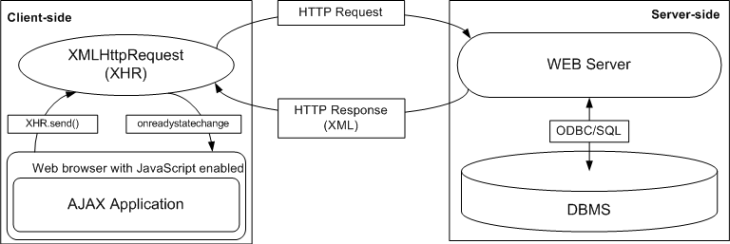
\includegraphics[width=0.8\textwidth]{./img/ajax01a.png}
		\caption{Example of an AJAX Architecture}
		\label{fig:ajax01}
	\end{center}
\end{figure}


It should be noted that AJAX has several shortcomings as well. First of all, 
JavaScript must be enabled in the browser, otherwise the application will not start.
However, the developer can indicate this in the \verb=<noscript>= HTML-tag. 
Nevertheless, the biggest issue with AJAX remains the fact that it is not a
standard. This often requires writing a different code base for different
browsers, and this means less scalability for the application and less productivity for
the developers~\cite{bgwt2}. In the latter case we could avoid some of the issues by using 
Google Web Toolkit (GWT).

\subsection{GWT}
\label{sec:gwt}

GWT is an open source project
and it is developed by Google. It is a set of tools and libraries that allows Web developers to
create AJAX applications in Java. 

The most important component of GWT is the Java-to-JavaScript compiler. It enables the
translation of Java code into highly optimized, browser independent
\footnote{As of GWT version 2.0, GWT supports: 
Firefox 1,~2,~3; Internet Explorer 6,~7,~8; Safari 2,~3,~4; Opera~9,~10, Chrome 1,~2,~3,~4, including mobile browsers for Android and the iPhone.} 
JavaScript code.
In addition to this, it provides developers with compile-time error checking. Another
very important aspect of the compiler is the fact that when the code is compiled into
JavaScript, it results in a single JavaScript file for each browser type and target locale.
This is illustrated in Figure~\ref{fig:gwt01}, which is an adaptation of~\cite[Figure 7]{wgio2}. 
Thus the client downloads and executes only the code that is specifically designed for that platform.  

\begin{figure}[ht]
	\begin{center}
		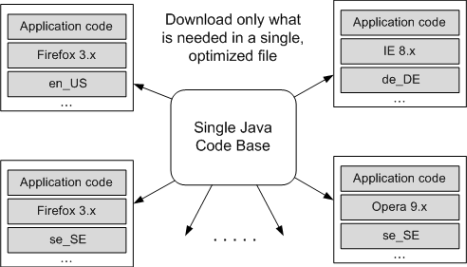
\includegraphics[width=0.8\textwidth]{./img/gwt01a.png}
		\caption{GWT Java-to-JavaScript Compiler}
		\label{fig:gwt01}
	\end{center}
\end{figure}

For additional literature on the subject of GWT, we recommend the book~\cite{bgwt2}. 
It has
proven to be very useful information source throughout the development process 
of LDBN. 

\subsection{Bitmap Rendering with JavaScript}
\label{sec:renderingJS}
When it comes to visualization and graphics in general a more low-level 
pixel control over a certain area of the screen is desired. 
When using JavaScript, however, simple tasks such as drawing a straight
line can become quite challenging in a Web browser environment.
Of course for this purpose we could use client-side solutions, e.g., 
using Flash, or server-side solution, e.g., 
rendering everything on the server as a static image 
and sending it back
to the client. However, for the same reasons as described in the previous
section we decided to use the AJAX approach. This way we can also
adopt a lot of the source code from the previous version of LDBN. 
One way to achieve bitmap rendering with JavaScript is by
using the \verb=<canvas>= HTML-element. 
It is part of the HTML5~\cite{html5} standard, which is the next major revision of HTML, and it is supported by
most of the modern Web browsers. It provides an image-like 
graphics context which can be accessed via a set of JavaScript calls, 
similar to a 2D subset of OpenGL. 
It was originally introduced by Apple in their Safari browser, but it is now 
supported by other modern browser including Mozilla Firefox, Opera and Google Chrome.
It also has better rendering speed than the older Scalable Vector Graphics (SVG) standard~\cite{w8}. 
Unfortunately, Internet Explorer (IE) provides native support for 
neither SVG nor canvas feature of HTML~\cite{w9}. In spite of that, IE does 
implements its own XML-based language for producing vector graphics 
called Vector Markup Language (VML). With the help of VML canvas-specific JavaScript 
calls can be emulated in IE. In LDBN we use the GWT-Incubator project~\cite{gwtincubator}, which provides
browser-independent canvas implementation for GWT projects, thus 
it provides support for all major browsers including IE. 
It should be noted that by doing this
we lose some rendering speed in IE that generally comes in other browsers
with a native canvas implementation. 
On the other hand, in our implementation of the visualization of FDs we use only static scenes, i.e., 
no animation or any other intensive 
graphical operations. Therefore, in our opinion, VML is sufficient for our project. 

\section{Implementation}
\label{sec:implementation}
As mentioned earlier the implementation is divided into two parts: 
(1) Visualization of FDs and 
(2) improving the existing capabilities of the system.

\subsection{Visualization of FDs}
\label{sec:visualization}
On the one hand the visualization of FDs is to be the most significant 
part of the thesis. 
On the other hand this extension should not compromise the existing 
user interface of LDBN 1.0. Therefore we decided to
make the visualization available in a separate window in the browser. 
The visualization is then available for every field in LDBN 1.1 which 
holds a set of FDs. In these fields there is an 
icon (
\includegraphics[scale=0.6]{./img/eye.png}) in the upper right
corner, by clicking it we can open the visualization window.
The initial idea
was to implement it as a separate Web application, which can then be 
opened in its own 
browser pop-up window. However, there are two problems with this approach. The first one is
the fact that most of the modern browsers have a pop-up blocker and it is activated by default.
This could have a major negative impact on the usability of the system because there
is always a risk that the user might not notice the pop-up 
warning at all and hence the visualization. The second problem with this approach is 
the fact that we want the visualization to use the existing 
advanced capabilities of LDBN 1.0 such as drag and drop. 
This would have been nearly impossible, though, since
the two application would run in different JavaScript virtual machines for each
browser window. The way around this issue could be the use of a server
which communicates with both applications. However, 
this would make the drag and drop too slow for effective usage. 

In LDBN 1.1 we use a different approach. We implement our own 
JavaScript-based window package, since GWT does not offer one in its standard library.
With it we can create pop-up windows which exist within a browser window. 
An example of such a window is presented in Figure~\ref{fig:fd-visual-win}. 
Our approach eliminates the previously described problems. First,
the window is part of our JavaScript application and as such it does not 
trigger any bowser pop-up blockers. 
Second, the visualization and the LDBN system can directly share any 
JavaScript objects, since they run in the same virtual machine, 
this way they can interact in a very fast and efficient way. 
This is very similar to the pop-up dialogs used in the initial version of our learning environment (LDBN 1.0). 
These dialogs are provided in the standard widget library of GWT. 
However, they prove to be inconvenient for our needs, since once created and attached 
to the DOM they cannot be resized. On the other hand, we
need this kind of resize-window functionality since we want to offer the user
different zoom levels for the visualization, as well as the ability the user to resize the
visualization window, since they could become quite large and hide important parts of the user 
interface. Furthermore, with our implementation we have more powerful control over
the graphical representation of the window. This way for example we can add a close button (image)
in the upper right corner, which is a more intuitive way to interact with the UI.

\begin{figure}[ht]
	\begin{center}
		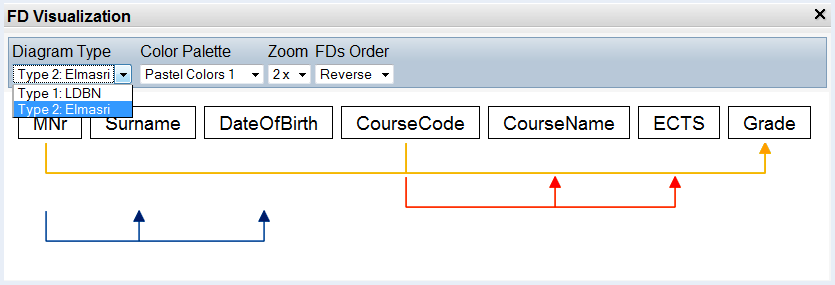
\includegraphics[width=0.9\textwidth]{./img/fd-visual-win.png}
		\caption{FD Visualization Window}
		\label{fig:fd-visual-win}
	\end{center}
\end{figure}

At the implementation level the visualization consists of two components. 
Both of them are illustrated in Figure~\ref{fig:impl-fds01}.
The first component is a simple GWT panel where all the attributes of an FD are displayed. 
Internally the attributes are represented as GWT widgets, thus the rendering of those attributes is
handled by the browser. In fact, these are the same widget classes used for representing
attributes in the \emph{Given Attributes} field, which is shown in Figure~\ref{fig:given-atts}. 
The only difference between the two kinds of attribute representations is 
that we apply a different CSS style sheet for each of them. By using the already implemented in LDBN 1.0 
widget classes we get advanced functionality such as drag and drop for free. Thus the user
can drag any attribute in the visualization window and drop 
it in the text box of the different editors in LDBN
such as the \emph{Attribute Editor} or the \emph{FD Editor}, the latter is 
shown in Figure~\ref{fig:fdeditor}. 
As a result the
attributes are automatically inserted in the text areas of the editor and users do not have
to type them by hand, which for long attribute names could become inconvenient and error prone. 
We believe the drag and drop functionality can help
users define attributes, keys or FDs much more quickly, which can
help improve the usability of the learning environment.

\begin{figure}[ht]
	\begin{center}
		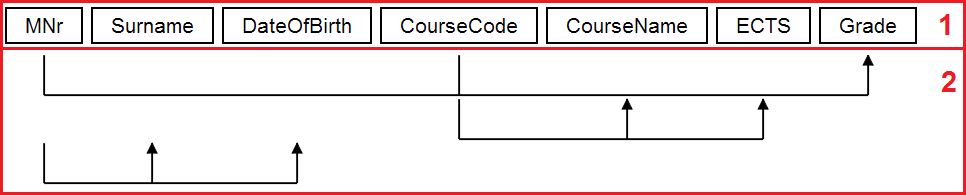
\includegraphics[width=0.9\textwidth]{./img/impl-fds01.png}
		\caption{Visualization Components}
		\label{fig:impl-fds01}
	\end{center}
\end{figure}

\begin{figure}[ht]
	\begin{center}
		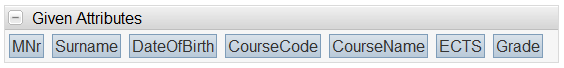
\includegraphics[width=0.9\textwidth]{./img/given-atts.png}
		\caption{Given Attributes Widget}
		\label{fig:given-atts}
	\end{center}
\end{figure}

\begin{figure}[ht]
	\begin{center}
		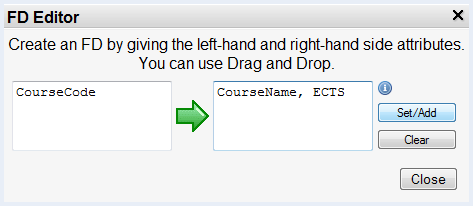
\includegraphics[width=0.6\textwidth]{./img/fdeditor.png}
		\caption{FD Editor Dialog in LDBN}
		\label{fig:fdeditor}
	\end{center}
\end{figure}

The second component of the visualization consists of a \verb=<canvas>= HTML5-element. 
It is shown in Figure~\ref{fig:impl-fds01}.
The canvas element is placed bellow the attributes, and there the actual drawing 
of the FDs takes place. In LDBN we support two types of visualization, each of them can be selected
from the \emph{Diagram Type} drop down menu in the visualization window. The first type is called 
\emph{Elmasri}, since it is the form of representation used in~\cite{bdb1}. 
The main difference between this approach and
the traditional representation of FDs is the fact the we display each attribute in the set of 
FDs only once. 
Similar to the purely text-based representation we can visualize the set
of FDs as a set of rows. Each row representing one FD of the set. 
However, in this visualization all attributes that occur in the set of FDs
are shown in the first row. Then every FD is displayed in a separate row by an outgoing 
arrow for each attribute from the left-hand side (LHS) of the FD,
and as an incoming arrow for the attributes of the right-hand side (RHS).

This approach is quite intuitive and we believe it will be well received by
students, since during their database courses at the university most of 
them get familiar with~\cite{bdb1}, from which
the visualization is inspired. However, the approach has some disadvantages
as well, not the least of which is the fact that it does not make use
of all the available white space in the diagram. To address this issue
we offer an option where the user can change the order in which
the FDs are rendered. In addition to this, we also offer another type of
visualization where the arrows of each FD always start/reach the 
attributes at the top of the diagram. 
Both types of visualization can be observed in 
Figure~\ref{fig:dia_example_elmasry} and~\ref{fig:dia_example_ldbn}.

\begin{figure}[ht]
  \centering
  \subfigure[Type: Elmasri]{
    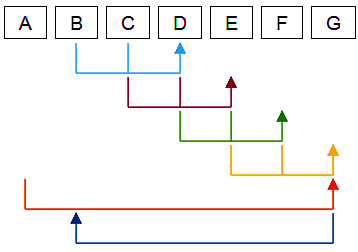
\includegraphics[scale=0.5]{./img/dia-elmasri-ex-fds-01.png}
    \label{fig:dia_example_elmasry}
  }
  \subfigure[Type: LDBN]{
    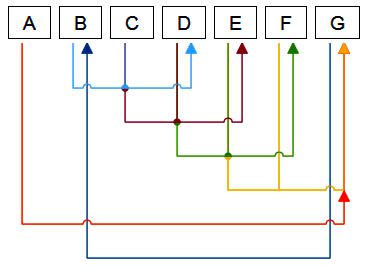
\includegraphics[scale=0.47]{./img/dia-ldbn-ex-fds-01.png}
    \label{fig:dia_example_ldbn}
  }
\caption{Diagram Types in LDBN}
\end{figure}

Certainly another important aspect in visualization in general are colors.
In our visualization we offer five different color palettes. The user can 
choose between:
\begin{enumerate}
	\item \emph{Black Only} - All FDs appear black. This is useful for printing
	purposes.
	\item \emph{Gray Shades} - Each FD appear in a different color tone of gray. 
	At this point is should be noted that when compared with other colors 
	the human eye can detect best shades of gray, and on a modern LCD screen it can
	distinguish between 30 shades of gray~\cite[Chapter 2]{bimg1} . 
	\item \emph{Pastel Colors} - Here we use less saturated colors which appear pastel. 
	Colors codes are taken from~\cite{wpastel}.
	\item \emph{Standard Colors} - The standard color palette consists of predefined
	HTML colors such as reg, green, blue, etc. These colors often appear vivid 
	(highly saturated colors).
	\item \emph{OpenOffice Style} - In this  palette we use colors which
	can be found in charts created with the help of OpenOffice.org~\cite{wooorg}. 
\end{enumerate}
 
% Color Contrast 
% see http://snook.ca/technical/colour_contrast/colour.html
% http://www.w3.org/WAI/WCAG20/quickref/#qr-visual-audio-contrast-contrast
% http://www.w3.org/TR/2008/NOTE-WCAG20-TECHS-20081211/G18

Another important issue when using colors is contrast. 
According to the W3C guidelines a Web application should use such
foreground and a background colors that provide enough of a
contrast \emph{``when viewed by someone having color deficits or when 
viewed on a black and white screen``}~\cite{w3c1}.
To ensure these property we use WCAG 2.0 contrast ratio formula~\cite{w3c2}.
Our color palettes are WCAG 2 AA Compliant for text larger than 18pt.

As can be seen in Figure~\ref{fig:fd-visual-win}, 
the visualization feature offers a magnification function as well. 
Thus the user can zoom in and out on a diagram.
This is practical especially when a
diagram contains a lot of attributes and the user 
wants to get a general idea of the FDs, then 
he\footnote{``He`` should be read as ``he or she`` throughout this thesis.} can
simply zoom out. 
The zoom functionality
is achieved by applying different CSS with different font 
size for the attributes and by redrawing the canvas element accordingly. 

\subsection{Improving the Usability of LDBN}
\label{sec:improving}

Another major part of this thesis is the improvement of the
existing functionality of the learning environment. 
To address some of the issues described in 
Section~\ref{sec:problem_statement} we introduced a more sophisticated user system in 
LDBN 1.1. In the previous version of the system all user had the same rights. 
In the current version we introduce following three groups of user:
(1) \emph{Regular Users}, (2) \emph{Instructional Users}, and (3) \emph{Superusers}.

Furthermore, each user group has different rights in the system. 
Table \ref{tab:user-rights} shows the different user rights in LDBN 1.1 for each user group. 

\begin{center}
\begin{table}
\begin{tabular}[h]{| m{2.8cm} || m{2.2cm} | m{3.2cm} | m{3.3cm} |}
\hline
 & \textbf{Regular Users} & \textbf{Instructional Users} & \textbf{Superusers} \\
\hline
\hline
\emph{Create \mbox{Assignments}} & Yes & Yes & Yes \\
\hline
\emph{Edit \mbox{Assignments}}  & Only their own & Their own and assignments submitted by regular users & Their own and assignments submitted by regular or instructional users \\
\hline
\emph{Delete \mbox{Assignments}} & No & Their own and assignments submitted by regular users & Their own and assignments submitted by regular regular or instructional users \\
\hline
\emph{Leave \mbox{Comments}}    & Yes & Yes & Yes \\
\hline
\emph{Edit \mbox{Comments}}     & Only their own & Their own and comments submitted by regular users & Their own and comments submitted by regular or instructional users\\
\hline
\emph{Delete \mbox{Comments}}   & Only their own & Their own and comments submitted by regular users & Their own and comments submitted by regular or instructional users \\
\hline
\emph{Add Users to the Group of \mbox{Instructional Users}} & No & Yes & Yes \\
\hline
\emph{Remove Users from the Group of \mbox{Instructional Users}} & No & No & Yes \\
\hline
\end{tabular}
\caption{User Rights in LDBN 1.1}
\label{tab:user-rights}
\end{table}
\end{center}


Under the hood LDBN manages the user data in a MySQL database. 
We realize the different user groups by simply altering the already existing table \verb=users=. 
and adding two more attributes 
of type boolean - \verb=isInstructionalUser= and \verb=isSuperuser=. 
These attributes are set to \verb=true= when a user has instructional user and respectively superuser 
rights in the system. 

Furthermore, in order to make it easier for instructional users and superusers to manage the system
we develop an extra user interface (UI) in LDBN called \emph{Administrators}, which is accessible via a
separate tab. It can be seen in Figure~\ref{fig:admin-ui}. 
The \emph{Administrators} UI offers three buttons which open 
different dialogs for adding/removing users to/from the instructional user group and for
deleting assignments. Creating and editing assignments can still be done in the 
\emph{Create Assignments} tab. Furthermore, superusers rights can only be realized by making
a corresponding SQL statement for a specific user. However, this is not an issue, since 
we do not expect the system to have more than one or two superusers. 

\begin{figure}[ht]
	\begin{center}
		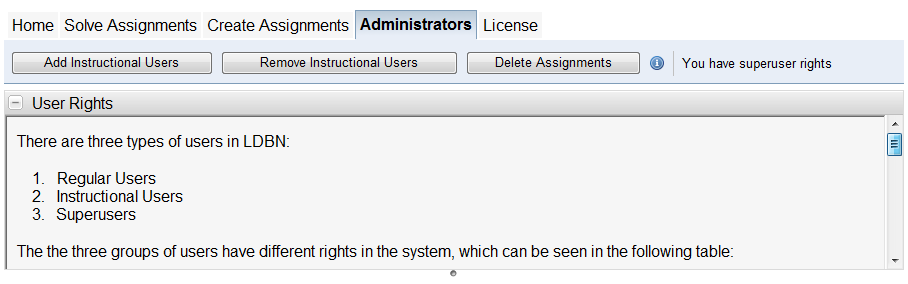
\includegraphics[width=0.9\textwidth]{./img/admin-ui.png}
		\caption{Administrators Tab}
		\label{fig:admin-ui}
	\end{center}
\end{figure}

With the new separation of users into groups we can easily overcome most of 
the issues surrounding user privileges described in the Section~\ref{sec:problem_statement}.
Most importantly, we implement different filters for the \emph{Load Assignment} dialog,
which can be seen in Figure~\ref{fig:load-assg}. Thus the user can choose from 
a drop-down menu to show only assignments submitted by instructional users 
(or superusers), the user himself or to show all assignments stored in the system. 
In addition, it should be noted that only assignments submitted
by instructional and superusers are visible by default, since instructional users are in most
cases course lecturers and they provide more sophisticated and 
well-thought-out assignments. 

In order to view other assignments, which are present in the system, 
one should choose a different filter from the drop-down menu. 
We implement the filters on the client-side, thus when a new filter is
applied we do not cause a new server interaction. Rather we apply them
on the initially received dataset, which holds all the meta data for each assignment.
As a result, the UI is very responsive to user input. 
In order to further increase the usability of the \emph{Load Assignment} dialog
we implement a column-soring function for it. As a result, users can click on
the different headers such as \emph{Name, Author and Last Modified} and sort the 
assignments correspondingly in an increasing or in a decreasing order. This is once
again done on the client side. 

\begin{figure}[ht]
	\begin{center}
		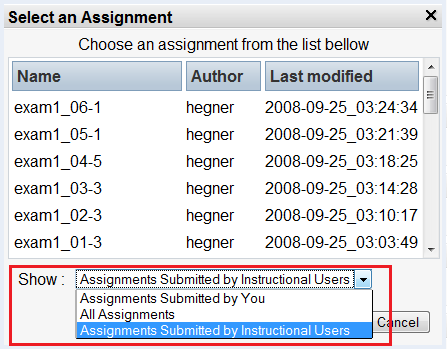
\includegraphics[width=0.6\textwidth]{./img/load-assg.png}
		\caption{Load Assignment Dialog with Filters}
		\label{fig:load-assg}
	\end{center}
\end{figure}

To decrease the number of assignments submitted to the system we added a new button
in the \emph{Create Assignments} tab called \emph{Load in SA Tab}, 
which can be observed in Figure~\ref{fig:load-in-sa}. 
In this case \emph{SA Tab} means \emph{``Solve Assignments Tab"},
which is the tab/view in the system, where students can test their knowledge by solving assignments. 
With the addition of this feature it is now possible to create an assignment and load it 
in the \emph{Solve Assignments} tab without
the need to first store it in the database. Moreover, users do not have to register or 
to log-in in order to use this
functionality. This new feature in LDBN 1.1 is especially useful for users who 
just want to get a general overview of the system and
do not want to become contributors, 
or for testing purposes for users who are currently creating an assignment. 

Another useful feature in LDBN 1.0 is the support for user comments, 
which users can give for each assignment. These comments
are then shown in the \emph{Solve Assignments} tab when the assignment is loaded. On the one
hand, such comments ensure that users can easily communicate and share ideas with each
other. On the other hand, comments could also decrease the amount of workload
for the lecturers in terms of giving an explanation to a difficult decomposition. However, in LDBN 1.0  
once submitted comments could not be altered. The only way to edit or to delete a
comment was to make the corresponding change directly in the database of the system. 
In the new version of our implementation (LDBN 1.1) 
users can edit and delete comments directly via the UI. When a user has
the rights to make a change on a comment or to delete it a corresponding icon is shown 
(
\includegraphics[scale=0.7]{./img/edit.png} or 
\includegraphics[scale=0.7]{./img/del.png})
next to the comment entry.

\begin{figure}[ht]
	\begin{center}
		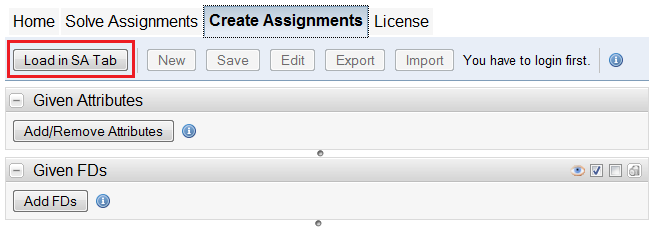
\includegraphics[width=0.75\textwidth]{./img/load-in-sa.png}
		\caption{Load in SA Tab Button}
		\label{fig:load-in-sa}
	\end{center}
\end{figure}
